\chapter{Atividade 2 -- Paralelismo em nível de instrução e otimizações do compilador}

\label{chap:atvd02}

\section{Enunciado da tarefa}

\label{sec:atvd02-enunciado}

\begin{quote}

Implemente três laços em C para investigar os efeitos do paralelismo em nível de instrução
(\textit{Instruction-Level Parallelism} -- ILP) e as possíveis otimizações realizadas pelo
compilador.

Os três casos devem inicializar um vetor utilizando um cálculo simples, somar seus elementos
de forma acumulativa criando dependência entre as iterações, e quebrar essa dependência
utilizando múltiplas variáveis de acumulação.

Compare o tempo de execução das versões compiladas com diferentes níveis de otimização:
\texttt{-O0}, \texttt{-O2} e \texttt{-O3}, utilizando diferentes tamanhos de vetor.

\end{quote}


\section{Objetivos e requisitos}

\label{sec:atvd02-objetivos}

A atividade teve como objetivo investigar experimentalmente a relação entre dependências de
dados, paralelismo em nível de instrução e otimizações realizadas pelo compilador em laços
implementados na linguagem C.

Mais especificamente, buscou-se observar como duas formas semanticamente equivalentes de
realizar uma redução sobre um vetor podem apresentar comportamentos diferentes em função da
quantidade de dependências existentes entre as instruções.

Foram estabelecidos os seguintes requisitos para o experimento:

\begin{itemize}
    \item implementar o experimento integralmente em C;
    \item utilizar o tipo \texttt{int} para o vetor e para as variáveis de acumulação;
    \item implementar um laço de inicialização do vetor;
    \item implementar uma redução com um único acumulador;
    \item implementar uma redução equivalente utilizando quatro acumuladores independentes;
    \item variar o tamanho \(N\) do vetor;
    \item compilar o mesmo código com \texttt{-O0}, \texttt{-O2} e \texttt{-O3};
    \item medir tempo decorrido utilizando \texttt{CLOCK\_MONOTONIC}, e não contadores de
    ciclos do processador;
    \item realizar aquecimentos antes das medições efetivas;
    \item realizar múltiplas medições e utilizar a mediana como estatística representativa;
    \item validar que as duas implementações de soma produzam o mesmo resultado;
    \item apresentar os resultados de forma simples e textual no terminal.
\end{itemize}


\section{Fundamentação conceitual}

\label{sec:atvd02-fundamentacao}

\subsection{Paralelismo em nível de instrução}

O paralelismo em nível de instrução, ou ILP, corresponde à possibilidade de um processador
executar ou manter simultaneamente em diferentes estágios múltiplas instruções pertencentes
ao mesmo fluxo de execução.

Diferentemente do paralelismo baseado em \textit{threads}, o ILP não exige que o programa
possua múltiplas linhas de execução. Um único fluxo sequencial pode conter instruções
independentes que sejam executadas de forma sobreposta por uma arquitetura superscalar.

Considere, por exemplo, duas operações independentes:

\begin{verbatim}
a = x + y;
b = z + w;
\end{verbatim}

A segunda operação não necessita do resultado produzido pela primeira. Dessa forma, a
arquitetura possui maior liberdade para escalonar ambas sobre diferentes recursos internos.

A situação muda quando existe uma dependência:

\begin{verbatim}
a = x + y;
b = a + z;
\end{verbatim}

Nesse caso, a segunda instrução somente pode prosseguir após a produção de \texttt{a}. A
latência da primeira operação passa a integrar o caminho crítico da execução.


\subsection{Dependências carregadas entre iterações}

O segundo laço da atividade realiza uma redução na forma

\begin{equation}
S_{i+1} = S_i + v_i,
\end{equation}

em que \(v_i\) representa o elemento do vetor processado na iteração \(i\).

Em C, sua forma conceitual é

\begin{verbatim}
sum += vector[i];
\end{verbatim}

A variável \texttt{sum} produz uma dependência entre iterações consecutivas:

\begin{center}
\texttt{sum0 -> sum1 -> sum2 -> sum3 -> sum4 -> ...}
\end{center}

Cada nova adição precisa do resultado calculado na iteração imediatamente anterior. Trata-se
de uma dependência verdadeira de dados, do tipo RAW (\textit{Read After Write}), carregada
entre iterações do laço.

Essa cadeia reduz a quantidade de operações de soma independentes disponíveis simultaneamente
para o processador.


\subsection{Quebra da cadeia de dependência}

Uma forma clássica de aumentar o ILP disponível consiste em utilizar múltiplos acumuladores.

Em vez de manter uma única cadeia,

\begin{center}
\texttt{S -> S -> S -> S -> S -> S}
\end{center}

podem ser criadas várias cadeias independentes:

\begin{verbatim}
S0 -> S0 -> S0
S1 -> S1 -> S1
S2 -> S2 -> S2
S3 -> S3 -> S3
\end{verbatim}

No experimento foram empregados quatro acumuladores:

\begin{verbatim}
sum0 += vector[i];
sum1 += vector[i + 1];
sum2 += vector[i + 2];
sum3 += vector[i + 3];
\end{verbatim}

Somente ao final as quatro somas parciais são combinadas.

Essa reorganização mantém o resultado lógico da redução, porém expõe operações independentes
que podem ser escalonadas de forma sobreposta pelo processador.


\subsection{ILP, desenrolamento de laços e vetorização}

A presença de múltiplas operações independentes também pode facilitar transformações
realizadas pelo compilador.

Entre as otimizações relacionadas a laços encontram-se o desenrolamento
(\textit{loop unrolling}), o reordenamento e escalonamento de instruções e a vetorização
SIMD.

É importante distinguir ILP de vetorização. ILP é um conceito mais amplo: diferentes
instruções escalares podem ser executadas simultaneamente ou de maneira sobreposta.
Vetorização, por outro lado, utiliza instruções capazes de operar sobre vários elementos
de dados de uma única vez.

Consequentemente, uma melhoria observada após a compilação com níveis agressivos de
otimização não pode ser atribuída automaticamente a uma única técnica sem analisar
o código gerado ou os relatórios do compilador.


\subsection{Efeito do nível de otimização}

O mesmo código-fonte foi compilado com três níveis:

\begin{description}
    \item[\texttt{-O0}] minimiza transformações de otimização e mantém maior proximidade
    entre o código-fonte e o código gerado;
    
    \item[\texttt{-O2}] habilita um conjunto amplo de otimizações consideradas adequadas
    para uso geral;
    
    \item[\texttt{-O3}] adiciona transformações mais agressivas, particularmente relevantes
    para laços, exposição de paralelismo e vetorização.
\end{description}

A comparação entre esses níveis permite investigar não apenas a estrutura manual dos laços,
mas também a capacidade do compilador de transformar o código.


\subsection{Hierarquia de memória}

O tamanho do vetor também influencia o desempenho.

Os dados utilizados por um programa transitam por diferentes níveis da hierarquia de memória,
que apresentam capacidades e latências distintas. Em termos simplificados:

\begin{center}
Registradores
\(\rightarrow\)
L1
\(\rightarrow\)
L2
\(\rightarrow\)
L3
\(\rightarrow\)
memória principal
\end{center}

Para vetores pequenos, uma parcela maior do conjunto de dados pode permanecer próxima ao
processador. À medida que \(N\) aumenta, cresce a pressão sobre os níveis de cache e sobre o
subsistema de memória.

Portanto, um ganho obtido por aumento de ILP pode tornar-se proporcionalmente menor quando
o custo de movimentação de dados passa a representar uma parcela maior do tempo total.


\section{Interpretação didática da tarefa}

\label{sec:atvd02-interpretacao}

A tarefa foi interpretada como uma investigação da cadeia causal

\begin{equation}
\text{estrutura do código}
\rightarrow
\text{dependências}
\rightarrow
\text{ILP disponível}
\rightarrow
\text{otimizações}
\rightarrow
\text{código de máquina}
\rightarrow
\text{tempo observado}.
\end{equation}

O primeiro laço representa um caso no qual cada posição do vetor pode ser calculada
independentemente.

O segundo representa deliberadamente uma redução com dependência serial entre iterações.

O terceiro mantém o mesmo objetivo matemático do segundo, porém reorganiza a computação de
forma a disponibilizar quatro cadeias de dependência independentes.

Assim, o experimento não consiste apenas em determinar qual versão é mais rápida. O interesse
principal está em observar em quais condições a exposição manual de ILP produz benefício e
como esse benefício se modifica quando o compilador recebe maior liberdade para transformar
o código.


\section{Modelagem da solução}

\label{sec:atvd02-modelagem}

\subsection{Estrutura geral}

Foi desenvolvido um único programa, \texttt{benchmark.c}, compilado três vezes a partir do
mesmo código-fonte.

As três compilações diferem pelo nível de otimização:

\begin{verbatim}
-O0
-O2
-O3
\end{verbatim}

Dessa forma, evita-se manter implementações diferentes para cada configuração e reduz-se o
risco de introduzir alterações acidentais entre os experimentos.

Para cada executável, o programa percorre internamente todos os valores de \(N\), executa
aquecimentos, realiza as medições, valida os resultados e apresenta as medianas no terminal.


\subsection{Inicialização do vetor}

O vetor foi inicializado de acordo com

\begin{equation}
v_i = (i \mathbin{\&} 7) + 1.
\end{equation}

Consequentemente, os elementos repetem a sequência

\begin{verbatim}
1 2 3 4 5 6 7 8
\end{verbatim}

Essa escolha possui três propriedades úteis para o experimento.

Primeiro, os elementos permanecem pequenos. Segundo, a soma esperada pode ser calculada
deterministicamente. Terceiro, mesmo para o maior vetor utilizado, a soma permanece abaixo do
limite representável por \texttt{int}.

Como

\begin{equation}
1+2+3+4+5+6+7+8=36,
\end{equation}

e todos os valores de \(N\) utilizados são múltiplos de oito, a soma esperada é

\begin{equation}
S_{\text{esperado}}=\frac{N}{8}\cdot 36.
\end{equation}


\subsection{Redução com acumulador único}

A implementação de referência emprega uma única variável:

\begin{verbatim}
int sum = 0;

for (size_t i = 0; i < n; ++i) {
    sum += vector[i];
}
\end{verbatim}

Essa versão apresenta diretamente a cadeia de dependência que constitui o principal objeto
de estudo da atividade.


\subsection{Redução com quatro acumuladores}

A segunda redução utiliza quatro somas parciais:

\begin{verbatim}
for (; i + 3 < n; i += 4) {
    sum0 += vector[i];
    sum1 += vector[i + 1];
    sum2 += vector[i + 2];
    sum3 += vector[i + 3];
}
\end{verbatim}

Ao final, calcula-se

\begin{equation}
S = S_0+S_1+S_2+S_3.
\end{equation}

Foi mantido ainda um laço residual para garantir a correção da função caso um tamanho que não
seja múltiplo de quatro seja utilizado futuramente.


\subsection{Principais funções e componentes}

A implementação foi decomposta nos seguintes componentes:

\begin{description}
    \item[\texttt{initialize\_vector()}] executa o primeiro laço e inicializa o vetor;
    
    \item[\texttt{sum\_single\_accumulator()}] executa a redução dependente;
    
    \item[\texttt{sum\_four\_accumulators()}] executa a redução com quatro cadeias
    independentes;
    
    \item[\texttt{measure\_initialization()}] mede somente a inicialização;
    
    \item[\texttt{measure\_single()}] mede somente a redução com acumulador único;
    
    \item[\texttt{measure\_multi4()}] mede somente a redução com quatro acumuladores;
    
    \item[\texttt{median()}] calcula a mediana das medições;
    
    \item[\texttt{expected\_sum()}] calcula o resultado esperado para validação;
    
    \item[\texttt{run\_for\_n()}] coordena todos os testes associados a um tamanho de vetor.
\end{description}


\section{Decisões de projeto e trade-offs}

\label{sec:atvd02-decisoes}

\subsection{Uso de \texttt{int}}

Foi utilizado \texttt{int} tanto para os elementos do vetor quanto para os acumuladores,
conforme definido para o experimento.

Essa decisão torna necessário controlar a possibilidade de \textit{overflow}. Por esse motivo,
foram escolhidos valores pequenos para os elementos do vetor e foi implementada uma verificação
do valor esperado.

Para o maior vetor,

\begin{equation}
N=16\,777\,216,
\end{equation}

a soma esperada é

\begin{equation}
75\,497\,472,
\end{equation}

valor amplamente inferior ao limite de um \texttt{int} de 32 bits utilizado no ambiente.


\subsection{Quatro acumuladores}

Foram utilizados quatro acumuladores independentes.

Um número maior poderia aumentar ainda mais o paralelismo explícito, mas também introduziria
maior pressão sobre registradores e transformaria a quantidade de acumuladores em uma nova
variável experimental.

Quatro acumuladores representam um compromisso entre simplicidade, clareza didática e
capacidade de exposição de ILP.


\subsection{Variação de \(N\)}

Foram utilizados os seguintes tamanhos:

\begin{table}[htbp]
    \centering
    \caption{Tamanhos de vetor utilizados no experimento.}
    \label{tab:atvd02-tamanhos}
    \begin{tabular}{r|r}
        \hline
        \(N\) & Memória ocupada pelo vetor \\
        \hline
        32\,768     & 128 KiB \\
        65\,536     & 256 KiB \\
        262\,144    & 1 MiB \\
        1\,048\,576 & 4 MiB \\
        2\,097\,152 & 8 MiB \\
        4\,194\,304 & 16 MiB \\
        16\,777\,216 & 64 MiB \\
        \hline
    \end{tabular}
\end{table}

Os tamanhos foram definidos em potências de dois e abrangem desde conjuntos de dados de
centenas de KiB até um vetor substancialmente maior que o cache de último nível informado
para a máquina.

Essa escolha permite observar tanto situações dominadas pela execução dos laços quanto
situações nas quais a movimentação de dados possui maior peso relativo.


\subsection{Mediana em vez de uma única execução}

Uma única medição está sujeita a interferências do sistema operacional, interrupções,
variações de frequência e processos concorrentes.

Foram utilizados três aquecimentos e vinte medições efetivas por configuração. O valor
reportado corresponde à mediana.

A mediana reduz a influência de observações isoladas anormalmente altas.


\subsection{Alternância da ordem das reduções}

Executar sempre a redução com acumulador único antes da versão com quatro acumuladores poderia
favorecer sistematicamente a segunda implementação por causa do estado da hierarquia de
memória.

Por esse motivo, a ordem foi alternada:

\begin{verbatim}
repetição par:    Single -> Multi4
repetição ímpar:  Multi4 -> Single
\end{verbatim}

A alternância não elimina todos os efeitos de cache, mas reduz um viés sistemático simples
entre as duas versões.


\subsection{Ausência de \texttt{-march=native}}

Embora a máquina tenha apresentado suporte a AVX, AVX2 e outras extensões durante a
caracterização inicial, \texttt{-march=native} não foi utilizado no experimento principal.

A intenção foi manter como principal variável de compilação apenas o nível de otimização:

\begin{verbatim}
-O0
-O2
-O3
\end{verbatim}

Adicionar \texttt{-march=native} criaria uma segunda variável, relacionada ao conjunto de
instruções disponível para geração de código.


\subsection{Uso de \texttt{noinline}}

As funções correspondentes aos laços foram marcadas para evitar \textit{inlining}.

Essa decisão facilita a separação conceitual dos experimentos e uma eventual inspeção do
código de máquina de cada função.

Como contrapartida, existe um pequeno custo de chamada de função, particularmente relevante
para os menores tamanhos de vetor. Esse efeito é discutido posteriormente entre as ameaças
à validade.


\section{Representação estrutural da implementação}

\label{sec:atvd02-estrutura}

A Figura~\ref{fig:atvd02-estrutura} resume a organização do experimento.

\begin{figure}[htbp]
\centering

\begin{tikzpicture}[
    node distance=8mm and 13mm,
    box/.style={
        draw,
        rounded corners,
        align=center,
        minimum width=27mm,
        minimum height=9mm
    },
    arrow/.style={-{Latex[length=2mm]}, thick}
]

\node[box] (src) {\texttt{benchmark.c}};

\node[box, below left=of src] (o0) {\texttt{-O0}};
\node[box, below=of src] (o2) {\texttt{-O2}};
\node[box, below right=of src] (o3) {\texttt{-O3}};

\node[box, below=17mm of o2] (n) {7 valores\\de \(N\)};

\node[box, below left=of n] (l1) {Loop 1\\Inicialização};
\node[box, below=of n] (l2) {Loop 2\\Single};
\node[box, below right=of n] (l3) {Loop 3\\Multi4};

\node[box, below=16mm of l2] (clock) {\texttt{CLOCK\_MONOTONIC}};
\node[box, below=of clock] (median) {20 medições\\mediana};
\node[box, below=of median] (out) {Resultado textual\\no terminal};

\draw[arrow] (src) -- (o0);
\draw[arrow] (src) -- (o2);
\draw[arrow] (src) -- (o3);

\draw[arrow] (o0) -- (n);
\draw[arrow] (o2) -- (n);
\draw[arrow] (o3) -- (n);

\draw[arrow] (n) -- (l1);
\draw[arrow] (n) -- (l2);
\draw[arrow] (n) -- (l3);

\draw[arrow] (l1) -- (clock);
\draw[arrow] (l2) -- (clock);
\draw[arrow] (l3) -- (clock);

\draw[arrow] (clock) -- (median);
\draw[arrow] (median) -- (out);

\end{tikzpicture}

\caption{Representação estrutural do experimento de ILP.}
\label{fig:atvd02-estrutura}
\end{figure}


\section{Fluxo de execução}

\label{sec:atvd02-fluxo}

Para cada valor de \(N\), a execução segue o fluxo apresentado na
Figura~\ref{fig:atvd02-fluxo}.

\begin{figure}[htbp]
\centering

\begin{tikzpicture}[
    node distance=7mm,
    box/.style={
        draw,
        rounded corners,
        align=center,
        minimum width=47mm,
        minimum height=8mm
    },
    arrow/.style={-{Latex[length=2mm]}, thick}
]

\node[box] (alloc) {Alocar vetor};
\node[box, below=of alloc] (touch) {\texttt{memset}: materializar páginas};
\node[box, below=of touch] (warm) {3 aquecimentos};
\node[box, below=of warm] (init) {Medir inicialização};
\node[box, below=of init] (sums) {Medir Single e Multi4\\alternando a ordem};
\node[box, below=of sums] (validate) {Validar resultados};
\node[box, below=of validate] (repeat) {Repetir até 20 medições};
\node[box, below=of repeat] (median) {Calcular medianas e speedup};
\node[box, below=of median] (print) {Exibir linha no terminal};
\node[box, below=of print] (free) {Liberar vetor};

\draw[arrow] (alloc) -- (touch);
\draw[arrow] (touch) -- (warm);
\draw[arrow] (warm) -- (init);
\draw[arrow] (init) -- (sums);
\draw[arrow] (sums) -- (validate);
\draw[arrow] (validate) -- (repeat);
\draw[arrow] (repeat) -- (median);
\draw[arrow] (median) -- (print);
\draw[arrow] (print) -- (free);

\end{tikzpicture}

\caption{Fluxo de execução para cada tamanho de vetor.}
\label{fig:atvd02-fluxo}
\end{figure}


\section{Metodologia experimental}

\label{sec:atvd02-metodologia}

\subsection{Ambiente de execução}

O experimento foi executado em uma máquina com as características apresentadas na
Tabela~\ref{tab:atvd02-ambiente}.

\begin{table}[htbp]
    \centering
    \caption{Características do ambiente utilizado no experimento.}
    \label{tab:atvd02-ambiente}
    \begin{tabular}{l|l}
        \hline
        Componente & Configuração \\
        \hline
        Processador & Intel Core i5-10300H @ 2,50 GHz \\
        Núcleos físicos & 4 \\
        Processadores lógicos & 8 \\
        L2 reportada pelo sistema & 1024 KiB \\
        L3 reportada pelo sistema & 8192 KiB \\
        Memória RAM & 31,84 GiB \\
        Memória configurada & 2667 MHz \\
        Sistema operacional & Windows 11 64 bits \\
        Plano de energia & Alto desempenho \\
        Compilador identificado & GCC 15.1.0 \\
        Tipo utilizado & \texttt{int}, 4 bytes \\
        \hline
    \end{tabular}
\end{table}

Durante a caracterização inicial, o compilador também reportou tamanho de linha de cache de
64 bytes e parâmetro de cache L1 de 32 KiB.

A execução final apresentada nesta seção foi realizada a partir de um terminal MSYS2/UCRT64.

Como o \textit{target} específico do compilador não foi novamente consultado após a mudança
para esse terminal, esse detalhe não é utilizado como base para nenhuma conclusão sobre os
resultados.


\subsection{Configuração das medições}

As três versões foram compiladas com os comandos equivalentes a:

\begin{verbatim}
gcc -std=c11 -Wall -Wextra -O0 \
    -DOPT_LEVEL='"O0"' benchmark.c -o benchmark_O0.exe

gcc -std=c11 -Wall -Wextra -O2 \
    -DOPT_LEVEL='"O2"' benchmark.c -o benchmark_O2.exe

gcc -std=c11 -Wall -Wextra -O3 \
    -DOPT_LEVEL='"O3"' benchmark.c -o benchmark_O3.exe
\end{verbatim}

Nenhuma flag adicional de arquitetura foi acrescentada à matriz principal.

Cada configuração utilizou:

\begin{table}[htbp]
    \centering
    \caption{Parâmetros do protocolo de medição.}
    \label{tab:atvd02-medicao}
    \begin{tabular}{l|l}
        \hline
        Parâmetro & Valor \\
        \hline
        Aquecimentos & 3 \\
        Medições efetivas & 20 \\
        Estatística reportada & Mediana \\
        Relógio & \texttt{CLOCK\_MONOTONIC} \\
        Acumuladores da versão Multi4 & 4 \\
        Níveis de otimização & \texttt{-O0}, \texttt{-O2}, \texttt{-O3} \\
        Quantidade de valores de \(N\) & 7 \\
        \hline
    \end{tabular}
\end{table}

O tempo medido contém somente o trecho correspondente ao laço de interesse.

Alocação de memória, liberação, impressão, ordenação das amostras, cálculo da mediana e
validação dos resultados permanecem fora das regiões cronometradas.

Foi utilizado ainda um \textit{compiler barrier} com efeito sobre memória em torno das regiões
cronometradas, reduzindo a possibilidade de movimentação de operações através das fronteiras
de medição pelo compilador.

Antes do início dos aquecimentos, um \texttt{memset} percorre a região alocada. O objetivo é
materializar previamente as páginas utilizadas e reduzir a influência de faltas de página de
primeiro acesso sobre a inicialização cronometrada.


\subsection{Métrica de speedup}

A comparação direta entre as duas formas de redução foi definida como

\begin{equation}
\text{Speedup}_{\text{Multi4}}
=
\frac{T_{\text{Single}}}
     {T_{\text{Multi4}}}.
\end{equation}

Assim:

\begin{equation}
\text{Speedup}>1
\end{equation}

indica vantagem da versão com quatro acumuladores, enquanto

\begin{equation}
\text{Speedup}<1
\end{equation}

indica que a versão com acumulador único foi mais rápida.


\section{Código-fonte desenvolvido}

\label{sec:atvd02-codigo}

O código completo utilizado no experimento é apresentado na
Listagem~\ref{lst:atvd02-codigo}.

\lstinputlisting[
    style=codigoC,
    caption={Código-fonte da Atividade 2.},
    label={lst:atvd02-codigo}
]{../ATVD2/benchmark.c}


\section{Validação da implementação}

\label{sec:atvd02-validacao}

A validação foi realizada em dois níveis.

Primeiramente, após cada execução das reduções, os resultados de
\texttt{sum\_single\_accumulator()} e \texttt{sum\_four\_accumulators()} foram comparados
diretamente.

Em seguida, o valor foi confrontado com a soma analiticamente esperada:

\begin{equation}
S_{\text{esperado}}=\frac{N}{8}\cdot36.
\end{equation}

Para o maior tamanho,

\begin{align}
N &= 16\,777\,216,\\
S_{\text{esperado}}
&=
\frac{16\,777\,216}{8}\cdot36\\
&=
75\,497\,472.
\end{align}

As três execuções terminaram com

\begin{verbatim}
Status: OK
Sink: 75497472
\end{verbatim}

confirmando que as duas implementações produziram o mesmo resultado para todos os tamanhos
testados e que o maior caso produziu o valor esperado.

A variável \texttt{benchmark\_sink}, declarada como \texttt{volatile}, também assegura um
efeito observável para os resultados das reduções, reduzindo o risco de eliminação completa
do trabalho pelo compilador.


\section{Resultados experimentais}

\label{sec:atvd02-resultados}

\subsection{Resultados com \texttt{-O0}}

A Tabela~\ref{tab:atvd02-o0} apresenta os resultados obtidos sem otimização.

\begin{table}[htbp]
\centering
\caption{Resultados obtidos com \texttt{-O0}.}
\label{tab:atvd02-o0}
\small
\begin{tabular}{r|r|r|r|r}
\hline
\(N\) & Init (ms) & Single (ms) & Multi4 (ms) & Speedup \\
\hline
32\,768      & 0,058600 & 0,063750 & 0,023450 & 2,719 \\
65\,536      & 0,116500 & 0,127150 & 0,047600 & 2,671 \\
262\,144     & 0,465550 & 0,507800 & 0,187250 & 2,712 \\
1\,048\,576  & 1,866300 & 2,095650 & 0,831800 & 2,519 \\
2\,097\,152  & 3,760450 & 4,262400 & 1,716550 & 2,483 \\
4\,194\,304  & 8,255650 & 9,086550 & 4,330800 & 2,098 \\
16\,777\,216 & 30,736250 & 34,333000 & 14,028250 & 2,447 \\
\hline
\end{tabular}
\end{table}

A versão Multi4 foi mais rápida em todos os tamanhos, apresentando speedup entre
\(2{,}098\times\) e \(2{,}719\times\).


\subsection{Resultados com \texttt{-O2}}

Os resultados com \texttt{-O2} são apresentados na
Tabela~\ref{tab:atvd02-o2}.

\begin{table}[htbp]
\centering
\caption{Resultados obtidos com \texttt{-O2}.}
\label{tab:atvd02-o2}
\small
\begin{tabular}{r|r|r|r|r}
\hline
\(N\) & Init (ms) & Single (ms) & Multi4 (ms) & Speedup \\
\hline
32\,768      & 0,018800 & 0,016400 & 0,005500 & 2,982 \\
65\,536      & 0,024300 & 0,020100 & 0,006600 & 3,045 \\
262\,144     & 0,094200 & 0,080650 & 0,027350 & 2,949 \\
1\,048\,576  & 0,397600 & 0,351900 & 0,135200 & 2,603 \\
2\,097\,152  & 0,819450 & 0,810600 & 0,455900 & 1,778 \\
4\,194\,304  & 1,655500 & 1,678100 & 0,917700 & 1,829 \\
16\,777\,216 & 7,108050 & 7,179200 & 4,652300 & 1,543 \\
\hline
\end{tabular}
\end{table}

O maior speedup de toda a matriz foi observado em

\begin{equation}
N=65\,536,
\end{equation}

com

\begin{equation}
\text{Speedup}=3{,}045\times.
\end{equation}

Entretanto, a vantagem relativa diminuiu para os vetores maiores.


\subsection{Resultados com \texttt{-O3}}

A Tabela~\ref{tab:atvd02-o3} apresenta os resultados obtidos com otimização
\texttt{-O3}.

\begin{table}[htbp]
\centering
\caption{Resultados obtidos com \texttt{-O3}.}
\label{tab:atvd02-o3}
\small
\begin{tabular}{r|r|r|r|r}
\hline
\(N\) & Init (ms) & Single (ms) & Multi4 (ms) & Speedup \\
\hline
32\,768      & 0,005000 & 0,002600 & 0,003300 & 0,788 \\
65\,536      & 0,009900 & 0,005600 & 0,006800 & 0,824 \\
262\,144     & 0,038500 & 0,025150 & 0,028550 & 0,881 \\
1\,048\,576  & 0,168300 & 0,179950 & 0,198800 & 0,905 \\
2\,097\,152  & 0,651300 & 0,545700 & 0,606050 & 0,900 \\
4\,194\,304  & 1,380250 & 1,014250 & 1,043000 & 0,972 \\
16\,777\,216 & 5,765100 & 4,054550 & 4,271200 & 0,949 \\
\hline
\end{tabular}
\end{table}

O comportamento foi qualitativamente diferente dos níveis anteriores. Todos os valores de
speedup ficaram abaixo de \(1\), indicando que a implementação Single foi mais rápida que
Multi4 em todos os tamanhos testados com \texttt{-O3}.


\section{Visualização dos resultados}

\label{sec:atvd02-visualizacao}

A Figura~\ref{fig:atvd02-speedup} reúne os speedups das três compilações.

\begin{figure}[htbp]
\centering

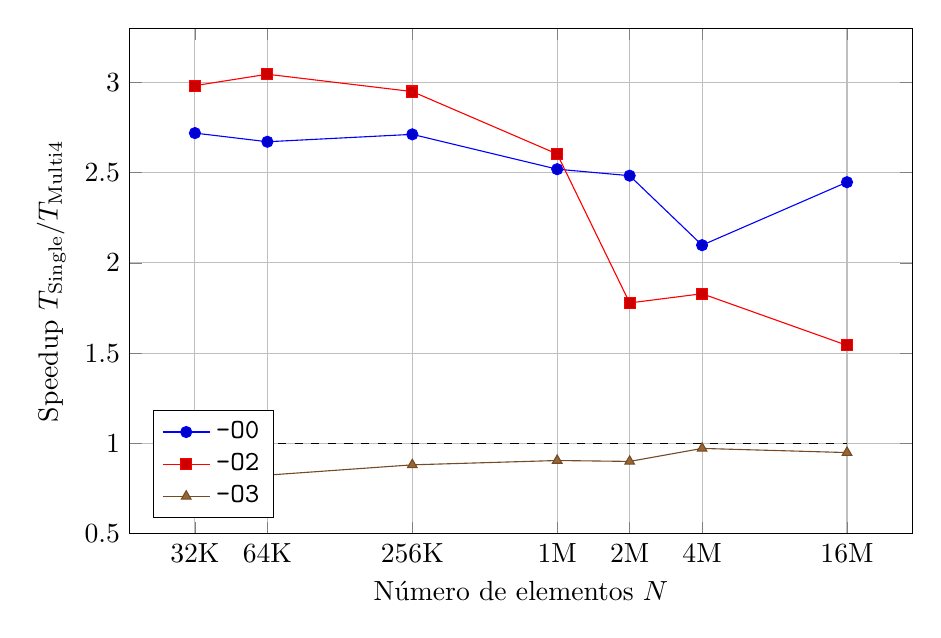
\begin{tikzpicture}

\begin{axis}[
    width=0.95\textwidth,
    height=8cm,
    xmode=log,
    log basis x=2,
    xlabel={Número de elementos \(N\)},
    ylabel={Speedup \(T_{\mathrm{Single}}/T_{\mathrm{Multi4}}\)},
    xtick={
        32768,
        65536,
        262144,
        1048576,
        2097152,
        4194304,
        16777216
    },
    xticklabels={
        32K,
        64K,
        256K,
        1M,
        2M,
        4M,
        16M
    },
    ymin=0.5,
    ymax=3.3,
    grid=both,
    legend pos=south west
]

\addplot+[mark=*] coordinates {
    (32768,2.719)
    (65536,2.671)
    (262144,2.712)
    (1048576,2.519)
    (2097152,2.483)
    (4194304,2.098)
    (16777216,2.447)
};
\addlegendentry{\texttt{-O0}}

\addplot+[mark=square*] coordinates {
    (32768,2.982)
    (65536,3.045)
    (262144,2.949)
    (1048576,2.603)
    (2097152,1.778)
    (4194304,1.829)
    (16777216,1.543)
};
\addlegendentry{\texttt{-O2}}

\addplot+[mark=triangle*] coordinates {
    (32768,0.788)
    (65536,0.824)
    (262144,0.881)
    (1048576,0.905)
    (2097152,0.900)
    (4194304,0.972)
    (16777216,0.949)
};
\addlegendentry{\texttt{-O3}}

\addplot[dashed, domain=32768:16777216] {1};

\end{axis}

\end{tikzpicture}

\caption{Speedup da implementação com quatro acumuladores em relação ao acumulador único. A linha tracejada em \(1\times\) representa igualdade de desempenho.}
\label{fig:atvd02-speedup}
\end{figure}

A inversão observada em \texttt{-O3} torna-se particularmente evidente: enquanto
\texttt{-O0} e \texttt{-O2} permanecem acima da linha de igualdade, todos os pontos de
\texttt{-O3} permanecem abaixo dela.

A Figura~\ref{fig:atvd02-maior-n} compara os tempos das duas reduções para o maior vetor.

\begin{figure}[htbp]
\centering

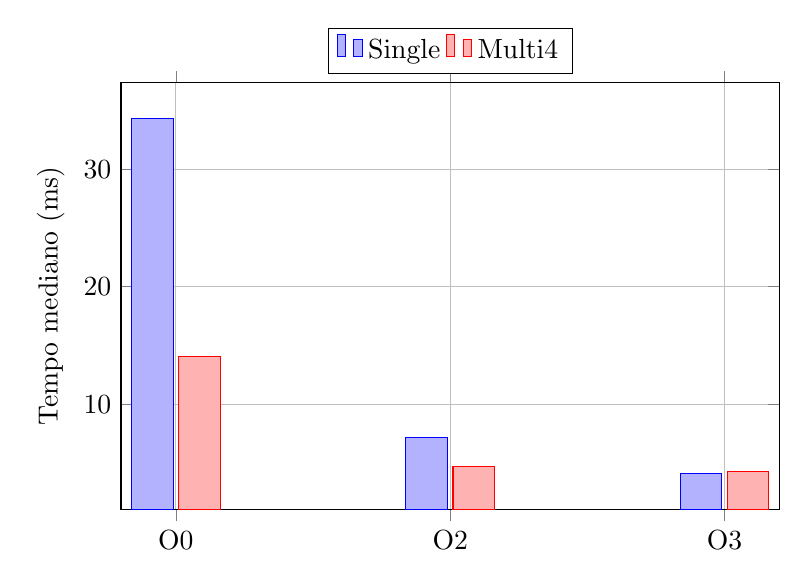
\begin{tikzpicture}

\begin{axis}[
    ybar,
    width=0.82\textwidth,
    height=7cm,
    bar width=15pt,
    ylabel={Tempo mediano (ms)},
    symbolic x coords={O0,O2,O3},
    xtick=data,
    legend style={at={(0.5,1.02)},anchor=south,legend columns=2},
    grid=major
]

\addplot coordinates {
    (O0,34.333000)
    (O2,7.179200)
    (O3,4.054550)
};

\addplot coordinates {
    (O0,14.028250)
    (O2,4.652300)
    (O3,4.271200)
};

\legend{Single,Multi4}

\end{axis}

\end{tikzpicture}

\caption{Tempos das duas reduções para \(N=16\,777\,216\) elementos (64 MiB).}
\label{fig:atvd02-maior-n}
\end{figure}


\section{Análise e discussão}

\label{sec:atvd02-discussao}

\subsection{Comportamento em \texttt{-O0}}

Os resultados de \texttt{-O0} apresentam de forma particularmente clara o efeito da
reestruturação manual.

A implementação com um acumulador obteve, para o primeiro tamanho,

\begin{equation}
T_{\text{Single}}=0{,}063750\text{ ms},
\end{equation}

enquanto Multi4 obteve

\begin{equation}
T_{\text{Multi4}}=0{,}023450\text{ ms},
\end{equation}

produzindo speedup de \(2{,}719\times\).

A vantagem permaneceu superior a \(2\times\) em todos os tamanhos.

Esse resultado é compatível com a fundamentação de ILP: a versão Single apresenta uma cadeia
de dependência contínua, enquanto Multi4 disponibiliza quatro cadeias independentes.

Em \texttt{-O0}, com menor intervenção do compilador sobre a estrutura original, a vantagem
da reorganização explícita torna-se especialmente visível.


\subsection{Comportamento em \texttt{-O2}}

Com \texttt{-O2}, Multi4 também foi mais rápida em todos os casos.

Para \(N=65\,536\), foram medidos:

\begin{align}
T_{\text{Single}} &= 0{,}020100\text{ ms},\\
T_{\text{Multi4}} &= 0{,}006600\text{ ms},
\end{align}

correspondendo a \(3{,}045\times\).

Nos três menores conjuntos de dados, o speedup permaneceu próximo de \(3\times\).

Entretanto, esse valor caiu progressivamente nos conjuntos maiores, chegando a
\(1{,}543\times\) para 64 MiB.

A redução da vantagem relativa é coerente com uma maior influência da hierarquia de memória
à medida que o \textit{working set} cresce.

No entanto, como não foram coletados contadores de hardware de \textit{cache miss},
largura de banda ou latência de memória, essa associação deve ser interpretada como
consistente com os resultados, e não como uma demonstração causal isolada.


\subsection{Inversão observada em \texttt{-O3}}

O resultado mais importante da atividade ocorreu com \texttt{-O3}.

Ao contrário de \texttt{-O0} e \texttt{-O2}, a versão com quatro acumuladores não apresentou
vantagem em nenhum tamanho.

Para \(N=32\,768\),

\begin{align}
T_{\text{Single}} &= 0{,}002600\text{ ms},\\
T_{\text{Multi4}} &= 0{,}003300\text{ ms},
\end{align}

resultando em speedup de apenas \(0{,}788\times\).

Mesmo para o maior vetor,

\begin{align}
T_{\text{Single}} &= 4{,}054550\text{ ms},\\
T_{\text{Multi4}} &= 4{,}271200\text{ ms},
\end{align}

com speedup de \(0{,}949\times\).

Portanto, a estrutura manualmente otimizada que apresentava vantagem de aproximadamente
duas a três vezes nos outros níveis deixou de ser a versão mais rápida quando foi utilizado
\texttt{-O3}.


\subsection{Efeito do compilador sobre a versão Single}

O maior vetor permite visualizar a magnitude das transformações associadas ao nível de
otimização.

Para Single:

\begin{align}
T_{\text{-O0}} &= 34{,}333000\text{ ms},\\
T_{\text{-O2}} &= 7{,}179200\text{ ms},\\
T_{\text{-O3}} &= 4{,}054550\text{ ms}.
\end{align}

A razão entre \texttt{-O0} e \texttt{-O3} é aproximadamente

\begin{equation}
\frac{34{,}333000}{4{,}054550}
\approx
8{,}47.
\end{equation}

Assim, para esse caso, a versão Single em \texttt{-O3} executou em aproximadamente
\(1/8{,}47\) do tempo registrado em \texttt{-O0}.

Para Multi4:

\begin{equation}
\frac{14{,}028250}{4{,}271200}
\approx
3{,}28.
\end{equation}

A versão manualmente reestruturada ainda se beneficiou de \texttt{-O3}, porém em proporção
consideravelmente menor.


\subsection{Interpretação da inversão}

Os resultados são compatíveis com a hipótese de que, em \texttt{-O3}, o compilador tenha
conseguido transformar agressivamente o laço Single, reduzindo a limitação representada pela
estrutura aparente do código-fonte.

Transformações possíveis incluem vetorização da redução, desenrolamento do laço, uso de
somas parciais internas e escalonamento de instruções.

Nesse cenário, a versão Single escrita no código-fonte não corresponde necessariamente a uma
única cadeia escalar de acumulação no código efetivamente executado.

Ao mesmo tempo, Multi4 já fornece explicitamente múltiplas cadeias, podendo existir menos
oportunidade para ganho adicional, além de maior complexidade estrutural e eventual pressão
sobre registradores.

Entretanto, os tempos medidos isoladamente não permitem afirmar qual transformação específica
foi aplicada.

Como os relatórios finais de vetorização e o \textit{assembly} das três funções não foram
utilizados nesta etapa da análise, a vetorização automática deve permanecer apresentada como
uma hipótese fortemente compatível com o comportamento observado, e não como fato
experimentalmente confirmado.


\subsection{Inicialização}

O primeiro laço também respondeu fortemente aos níveis de otimização.

Para o vetor de 64 MiB:

\begin{align}
T_{\text{Init,-O0}} &= 30{,}736250\text{ ms},\\
T_{\text{Init,-O2}} &= 7{,}108050\text{ ms},\\
T_{\text{Init,-O3}} &= 5{,}765100\text{ ms}.
\end{align}

A razão entre os extremos é

\begin{equation}
\frac{30{,}736250}{5{,}765100}
\approx
5{,}33.
\end{equation}

Como as iterações da inicialização escrevem posições distintas do vetor, não existe a mesma
dependência de redução presente no segundo laço. Essa estrutura oferece naturalmente mais
liberdade ao compilador para otimizações.


\subsection{Síntese dos comportamentos}

Os três níveis produziram padrões claramente distintos:

\begin{center}
\begin{tabular}{c|c}
\hline
Configuração & Comportamento observado \\
\hline
\texttt{-O0} & Multi4 entre \(2{,}098\times\) e \(2{,}719\times\) \\
\texttt{-O2} & Multi4 entre \(1{,}543\times\) e \(3{,}045\times\) \\
\texttt{-O3} & Single vence; speedup Multi4 entre \(0{,}788\times\) e \(0{,}972\times\) \\
\hline
\end{tabular}
\end{center}

Portanto, uma otimização manual benéfica em níveis menos agressivos não necessariamente
permanece superior após transformações mais avançadas realizadas pelo compilador.


\section{Limitações}

\label{sec:atvd02-limitacoes}

O experimento foi projetado para reduzir fontes simples de ruído, mas permanece sujeito a
limitações características de microbenchmarks executados em um sistema operacional de uso
geral.

A execução ocorreu no Windows 11, que continua realizando escalonamento, interrupções e
tarefas em segundo plano durante as medições.

O processador utilizado é um processador móvel. Sua frequência efetiva pode variar devido a
mecanismos de gerenciamento energético, \textit{turbo} e condições térmicas. O plano de
energia utilizado foi Alto desempenho, porém isso não garante frequência absolutamente
constante.

Não foi realizada afinidade explícita da execução com um núcleo específico.

Também não foram coletados contadores de desempenho de hardware. Consequentemente, as
associações entre mudanças de comportamento e níveis da hierarquia de cache não podem ser
tratadas como medições diretas de \textit{cache misses} ou largura de banda.

As funções dos laços foram marcadas como \texttt{noinline}. Isso facilita o isolamento e a
inspeção conceitual, mas mantém um custo de chamada que representa parcela proporcionalmente
maior nos casos mais curtos.

Esse ponto merece atenção especialmente em \texttt{-O3}, onde o menor tempo medido foi de

\begin{equation}
0{,}002600\text{ ms}=2{,}6\ \mu\text{s}.
\end{equation}

Por isso, as conclusões principais não dependem exclusivamente dos dois menores tamanhos de
vetor.

Por fim, os resultados permitem observar o efeito global do nível de otimização, mas não
identificam isoladamente quais passes do compilador produziram cada melhoria. Uma análise
posterior com relatório de vetorização e inspeção de \textit{assembly} seria necessária para
estabelecer essa relação de forma direta.


\section{Conclusões da atividade}

\label{sec:atvd02-conclusao}

A atividade demonstrou experimentalmente que dependências entre instruções possuem impacto
direto sobre o desempenho de laços e que a reorganização do código pode expor paralelismo em
nível de instrução.

Com \texttt{-O0}, a utilização de quatro acumuladores produziu speedups entre
\(2{,}098\times\) e \(2{,}719\times\), mostrando de forma clara o benefício da quebra da
cadeia de dependência.

Com \texttt{-O2}, a vantagem atingiu até \(3{,}045\times\), embora tenha diminuído à medida
que o tamanho do vetor cresceu.

O resultado mais relevante ocorreu em \texttt{-O3}. Nesse nível, a versão originalmente
dependente tornou-se mais rápida que a implementação manual com quatro acumuladores em todos
os tamanhos testados.

Esse comportamento evidencia que a estrutura do código-fonte não deve ser analisada
isoladamente do compilador. Um laço aparentemente serial no código C pode ser profundamente
transformado durante a otimização, enquanto uma transformação manual anteriormente vantajosa
pode tornar-se redundante ou menos eficiente.

A atividade também demonstrou a importância de uma metodologia experimental controlada.
Variação de \(N\), aquecimentos, múltiplas medições, mediana, alternância da ordem das
implementações, validação dos resultados e delimitação cuidadosa da região cronometrada foram
necessários para tornar a comparação mais robusta.

Assim, o principal resultado da atividade não é simplesmente que Multi4 ou Single seja a
melhor implementação. A conclusão é que o desempenho emerge da interação entre dependências
do algoritmo, exposição de ILP, hierarquia de memória e transformações realizadas pelo
compilador.


\section{Síntese}

\label{sec:atvd02-defesa}

Para uma defesa oral, os principais pontos da atividade podem ser sintetizados da seguinte
forma:

\begin{enumerate}
    \item \textbf{O que é ILP?} É a possibilidade de executar ou sobrepor instruções
    independentes dentro de um único fluxo de execução. Não é paralelismo por
    \textit{threads}.

    \item \textbf{Qual é o problema do acumulador único?} A instrução
    \texttt{sum += vector[i]} cria uma dependência RAW entre iterações. A próxima soma
    depende do resultado da anterior.

    \item \textbf{Por que quatro acumuladores ajudam?} Eles criam quatro cadeias independentes
    de dependência, disponibilizando mais operações simultaneamente para o processador.

    \item \textbf{Como o experimento foi medido?} Foram utilizados sete tamanhos de vetor,
    três aquecimentos, vinte medições por configuração, mediana e
    \texttt{CLOCK\_MONOTONIC}.

    \item \textbf{Por que variar \(N\)?} Para observar a execução em diferentes tamanhos de
    conjunto de dados e a mudança de importância relativa entre computação e hierarquia de
    memória.

    \item \textbf{O que aconteceu em \texttt{-O0}?} Multi4 foi de aproximadamente
    \(2{,}1\times\) a \(2{,}7\times\) mais rápida em termos da métrica de speedup utilizada.

    \item \textbf{O que aconteceu em \texttt{-O2}?} Multi4 continuou superior, chegando a
    \(3{,}045\times\), mas a vantagem diminuiu nos maiores vetores.

    \item \textbf{O que aconteceu em \texttt{-O3}?} O comportamento se inverteu. Single foi
    mais rápida em todos os tamanhos e os speedups de Multi4 ficaram abaixo de \(1\times\).

    \item \textbf{Por que \texttt{-O3} pode inverter o resultado?} Os dados são compatíveis
    com transformações agressivas realizadas pelo compilador, como vetorização,
    desenrolamento ou criação interna de somas parciais. Entretanto, o tempo sozinho não
    identifica qual transformação ocorreu.

    \item \textbf{Qual é a principal conclusão?} Uma otimização manual não deve ser julgada
    apenas pelo código-fonte. O resultado final depende da interação entre dependências,
    arquitetura, hierarquia de memória e código efetivamente produzido pelo compilador.

    \item \textbf{Como a correção foi validada?} Single e Multi4 foram comparadas entre si e
    com uma soma esperada calculada analiticamente. Todas as execuções terminaram com
    \texttt{Status: OK}.

    \item \textbf{Qual seria o próximo passo para aprofundar a análise?} Gerar os relatórios
    de vetorização do GCC e comparar o \textit{assembly} de Single e Multi4 em
    \texttt{-O0}, \texttt{-O2} e \texttt{-O3}, permitindo associar diretamente os tempos
    às transformações do compilador.
\end{enumerate}